\documentclass{beamer}

\usetheme{Madrid}
\usecolortheme{seagull}

\usepackage{graphicx}
\usepackage{tikz}
\usepackage{listings}
\usepackage{colortbl}

\tikzstyle{block} = [rectangle, draw, text width=4.5em, text centered, minimum height=2em]
\lstset{basicstyle=\small\ttfamily}



\lstset{
  language=Java,
  basicstyle=\ttfamily\small,
  keywordstyle=\color{blue},
  commentstyle=\color{green!60!black},
  stringstyle=\color{red},
  showstringspaces=false,
  breaklines=true
}

\setbeamertemplate{navigation symbols}{} % Remove navigation symbols

\title{Distributed Systems in Action}
\author{Mohamed Sweelam}
\institute{Software Engineer}
\date{}

\begin{document}

\begin{frame}
  \titlepage
\end{frame}

\begin{frame}{Outline}
  \tableofcontents
\end{frame}

\section{Introduction to Distributed Systems}
\begin{frame}{Introduction to Distributed Systems}
  \begin{itemize}
    \item Definition and characteristics of distributed systems
    \item Importance and benefits of distributed systems
    \item Challenges and trade-offs in designing distributed systems
  \end{itemize}
\end{frame}

\section{Use Case: Flight System}
\begin{frame}{Use Case: Flight System}
  \begin{center}
    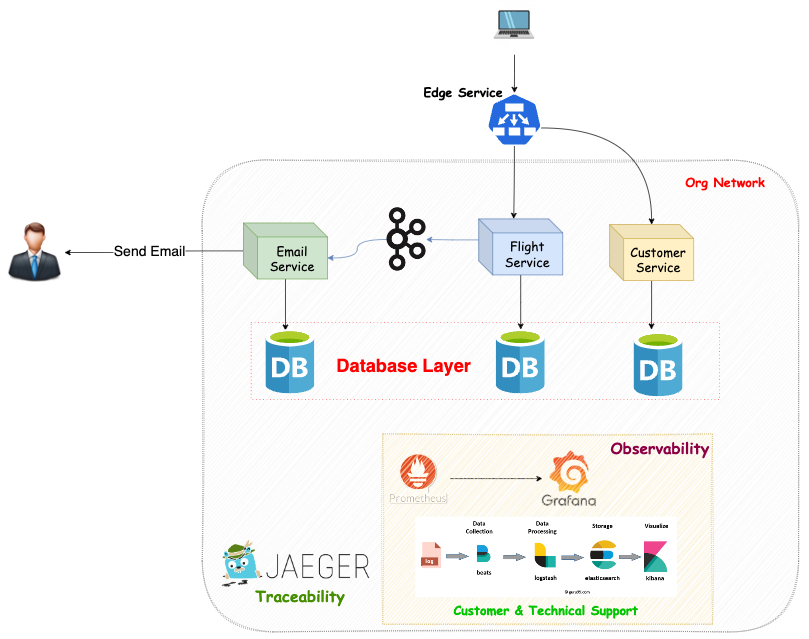
\includegraphics[width=0.7\textwidth]{img/system-HLD-1.png}
  \end{center}
\end{frame}

\section{CAP Theorem}
\begin{frame}{CAP Theorem}
  \begin{center}
    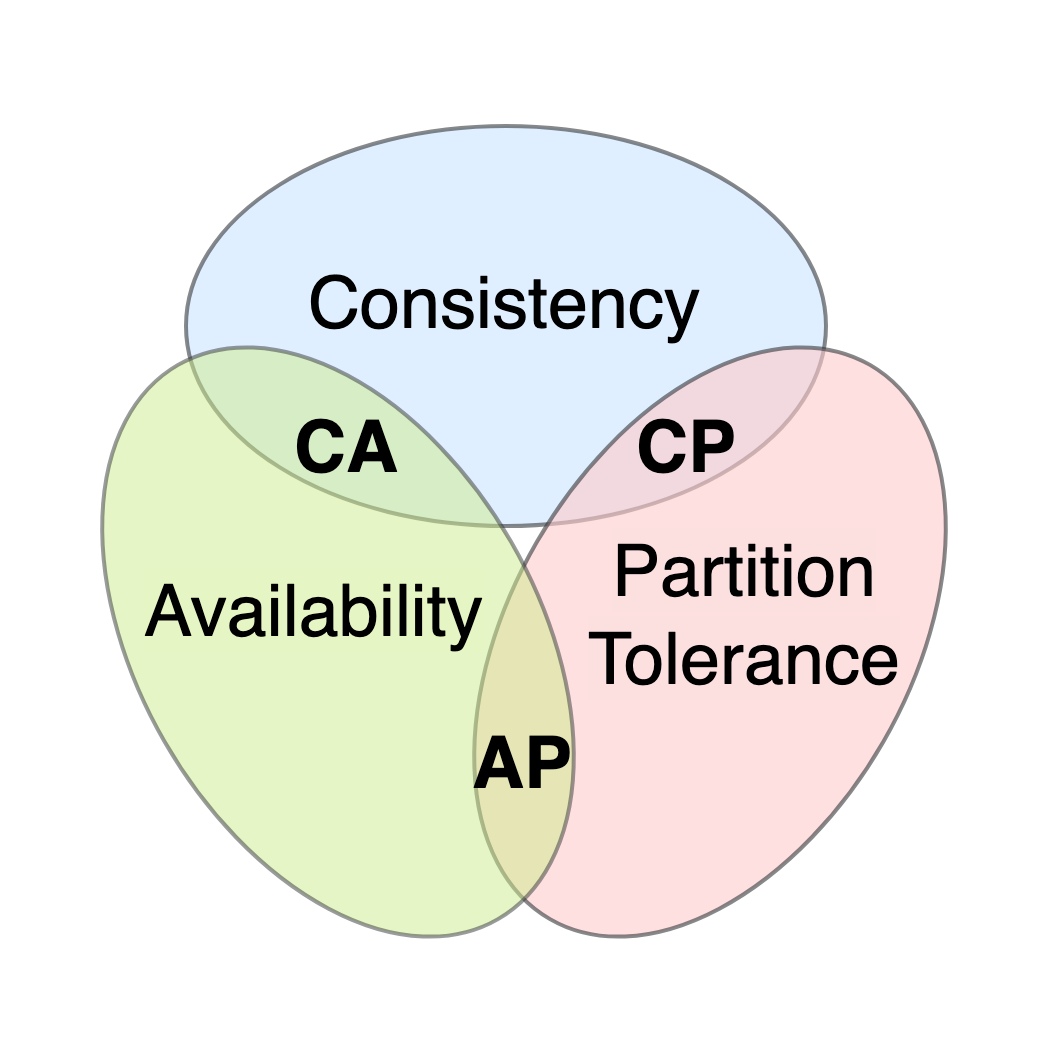
\includegraphics[width=0.7\textwidth]{img/CAP_Theorem_Venn_Diagram.png}
  \end{center}
\end{frame}

\section{Distributed Databases}
\begin{frame}{Distributed Databases}
	\begin{itemize}
    		\item \textbf{Consistency} every read operation gives a result of the most recent write.
    		\item \textbf{Availability} every read operation gives a non-error response, but, data might be staled.
    		\item \textbf{Partition Tolerance} system operates normally despite network failure.
    	\end{itemize}
  \begin{center}
    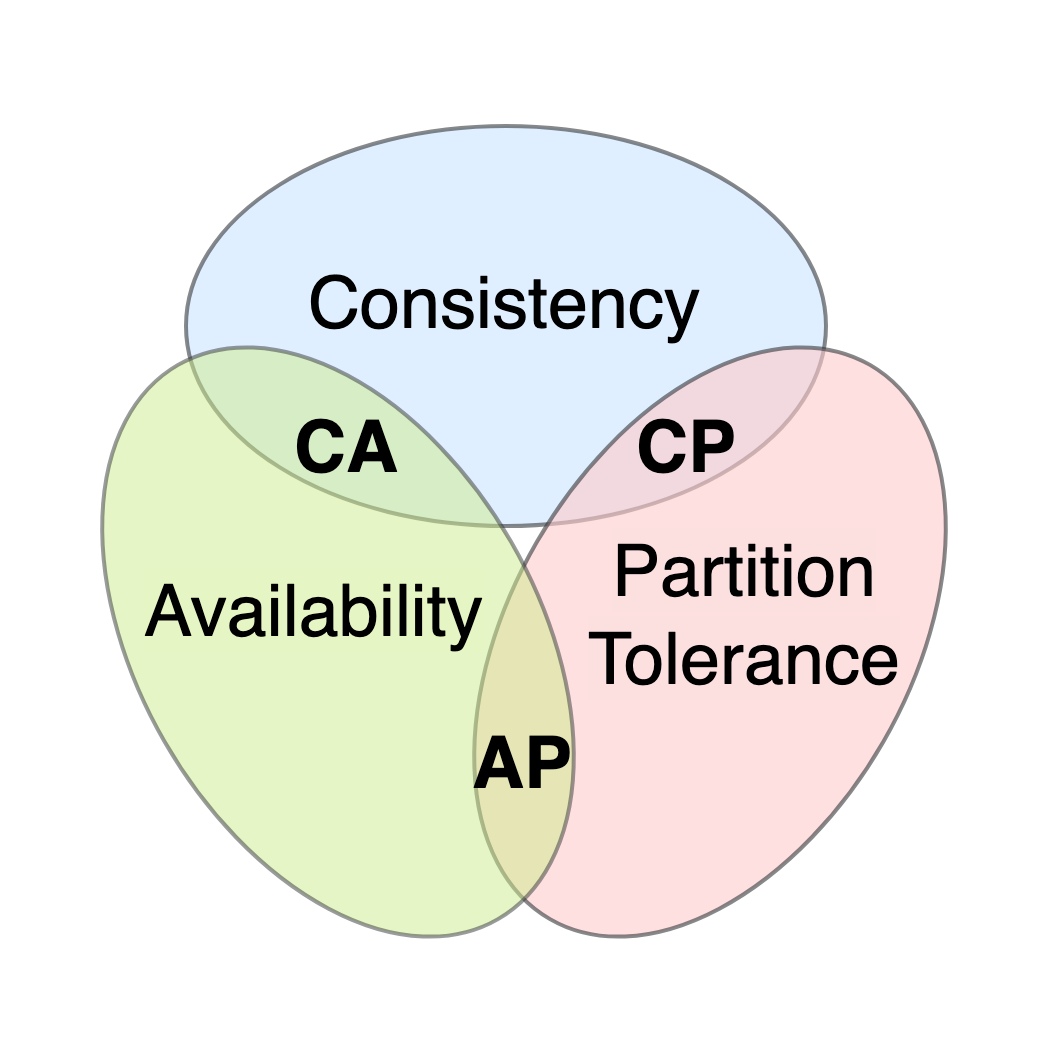
\includegraphics[width=0.3\textwidth]{img/CAP_Theorem_Venn_Diagram.png}
  \end{center}
\end{frame}


\begin{frame}{Distributed Databases}
  \begin{center}
    In the presence of network partitioning, system designers must choose between data consistency and availablity. \\
    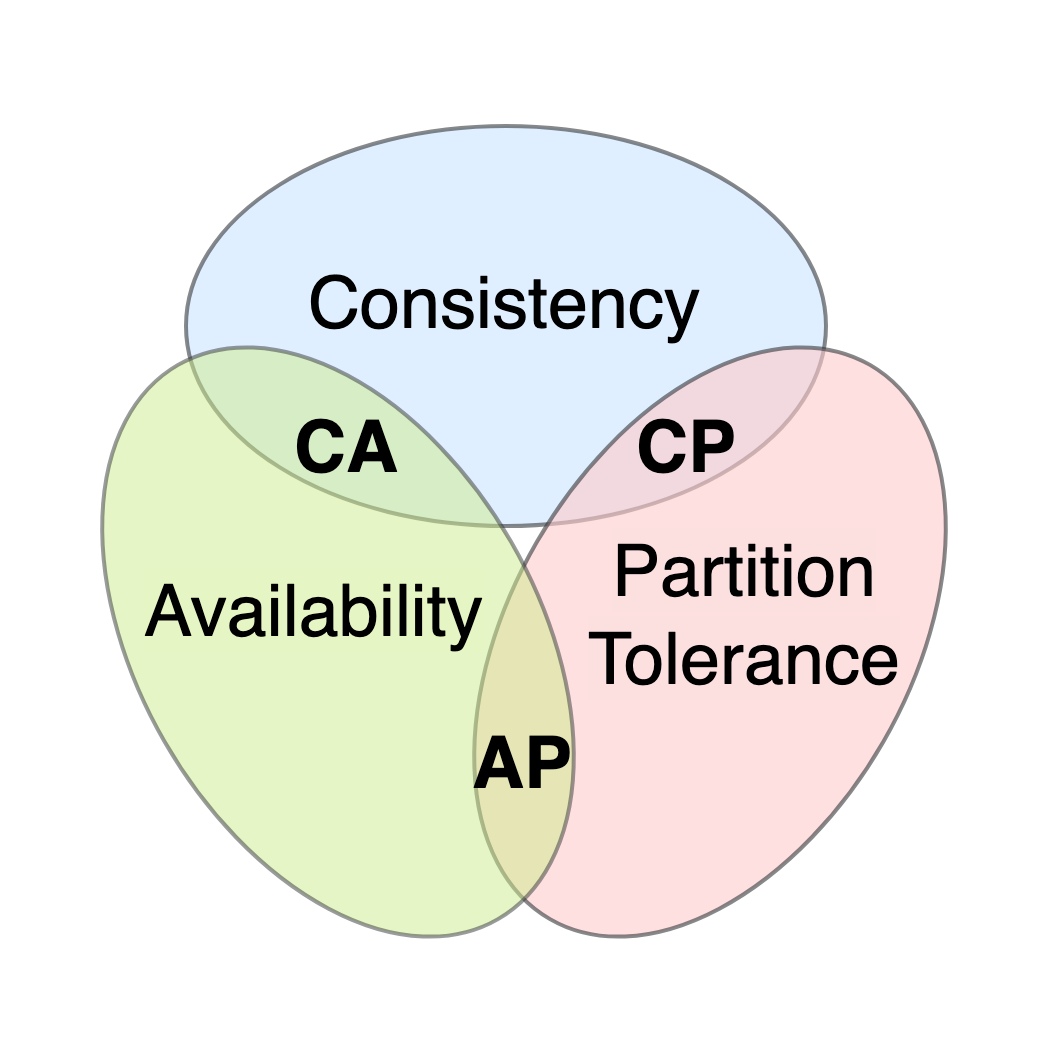
\includegraphics[width=0.5\textwidth]{img/CAP_Theorem_Venn_Diagram.png}
  \end{center}
\end{frame}


\begin{frame}{Distributed Databases}
  \begin{center}
    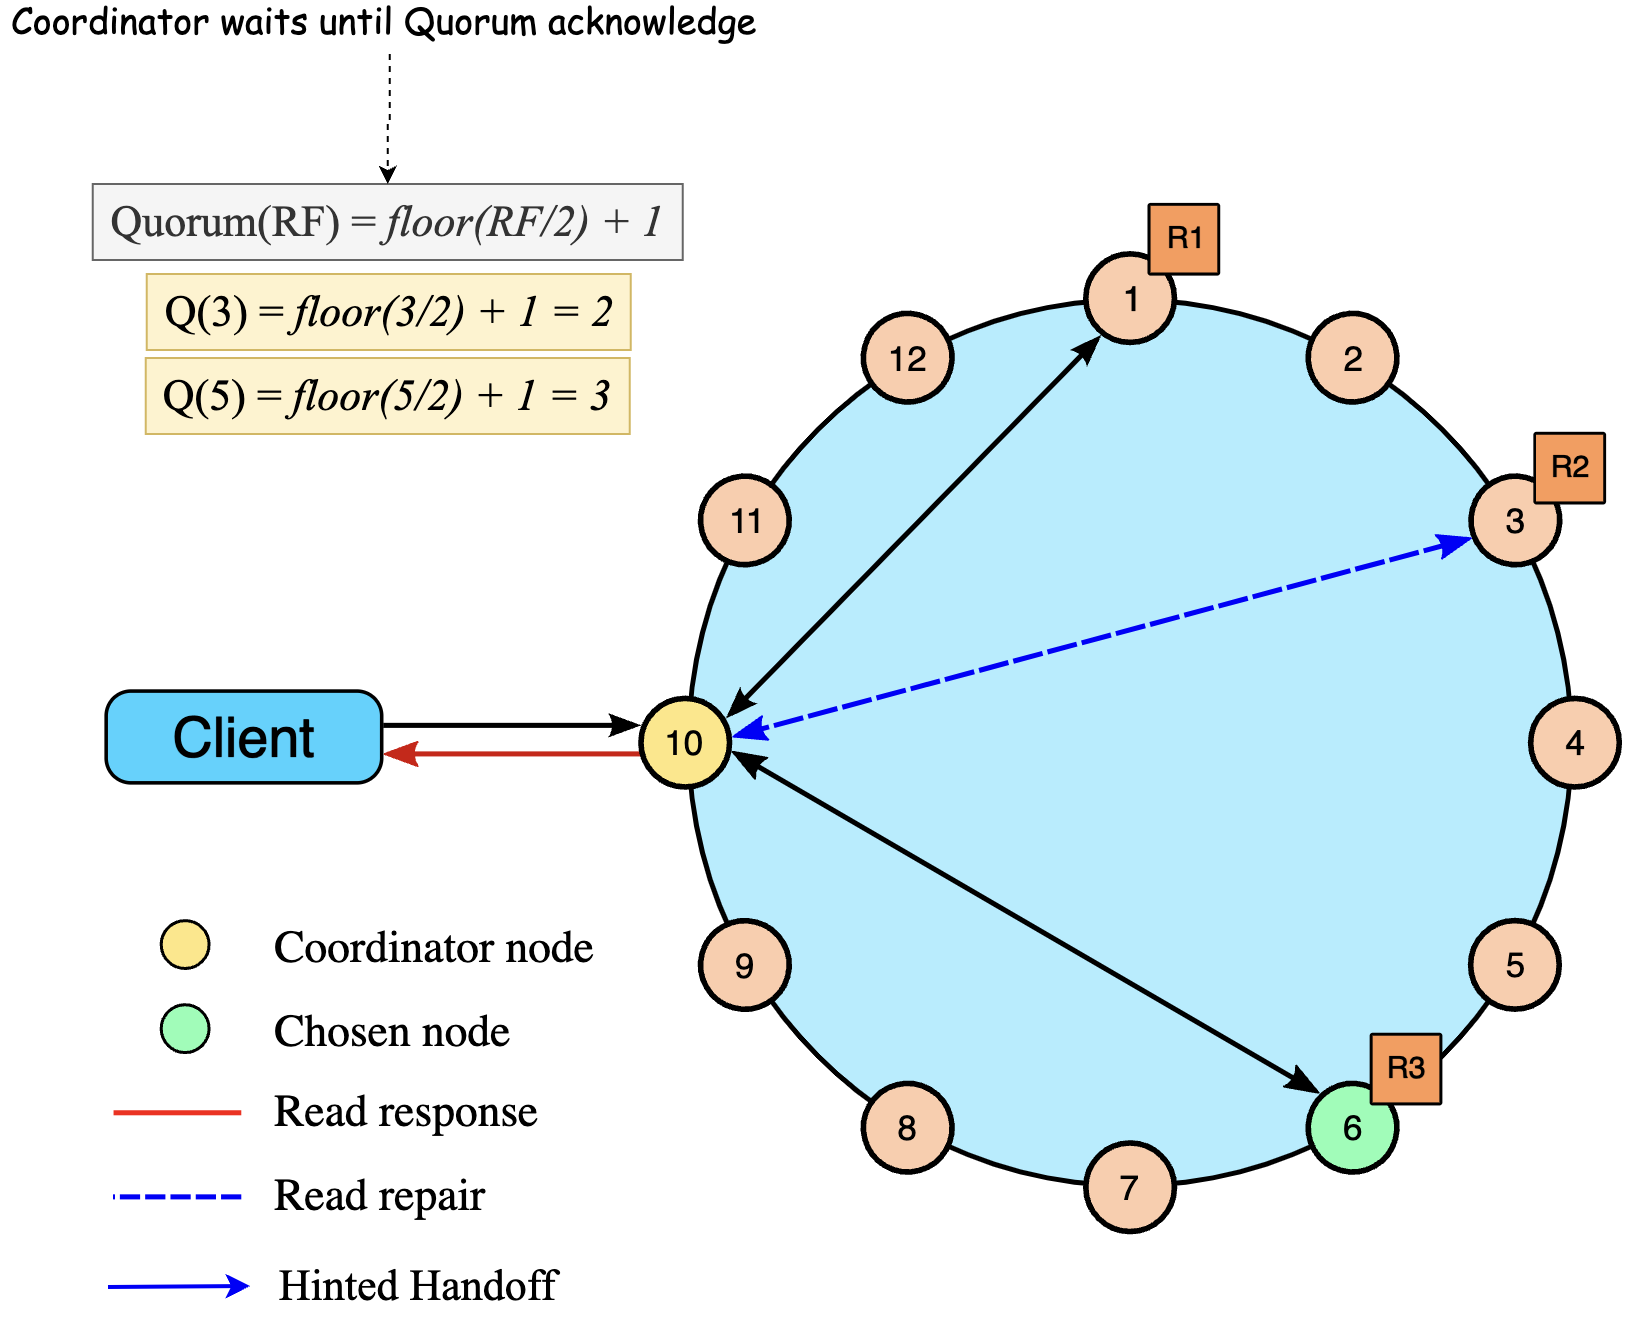
\includegraphics[width=0.8\textwidth]{img/Q-scenario.png}
  \end{center}
  
  Snapshot from Datastax website
\end{frame}


\begin{frame}{Distributed Databases}
  \begin{center}
    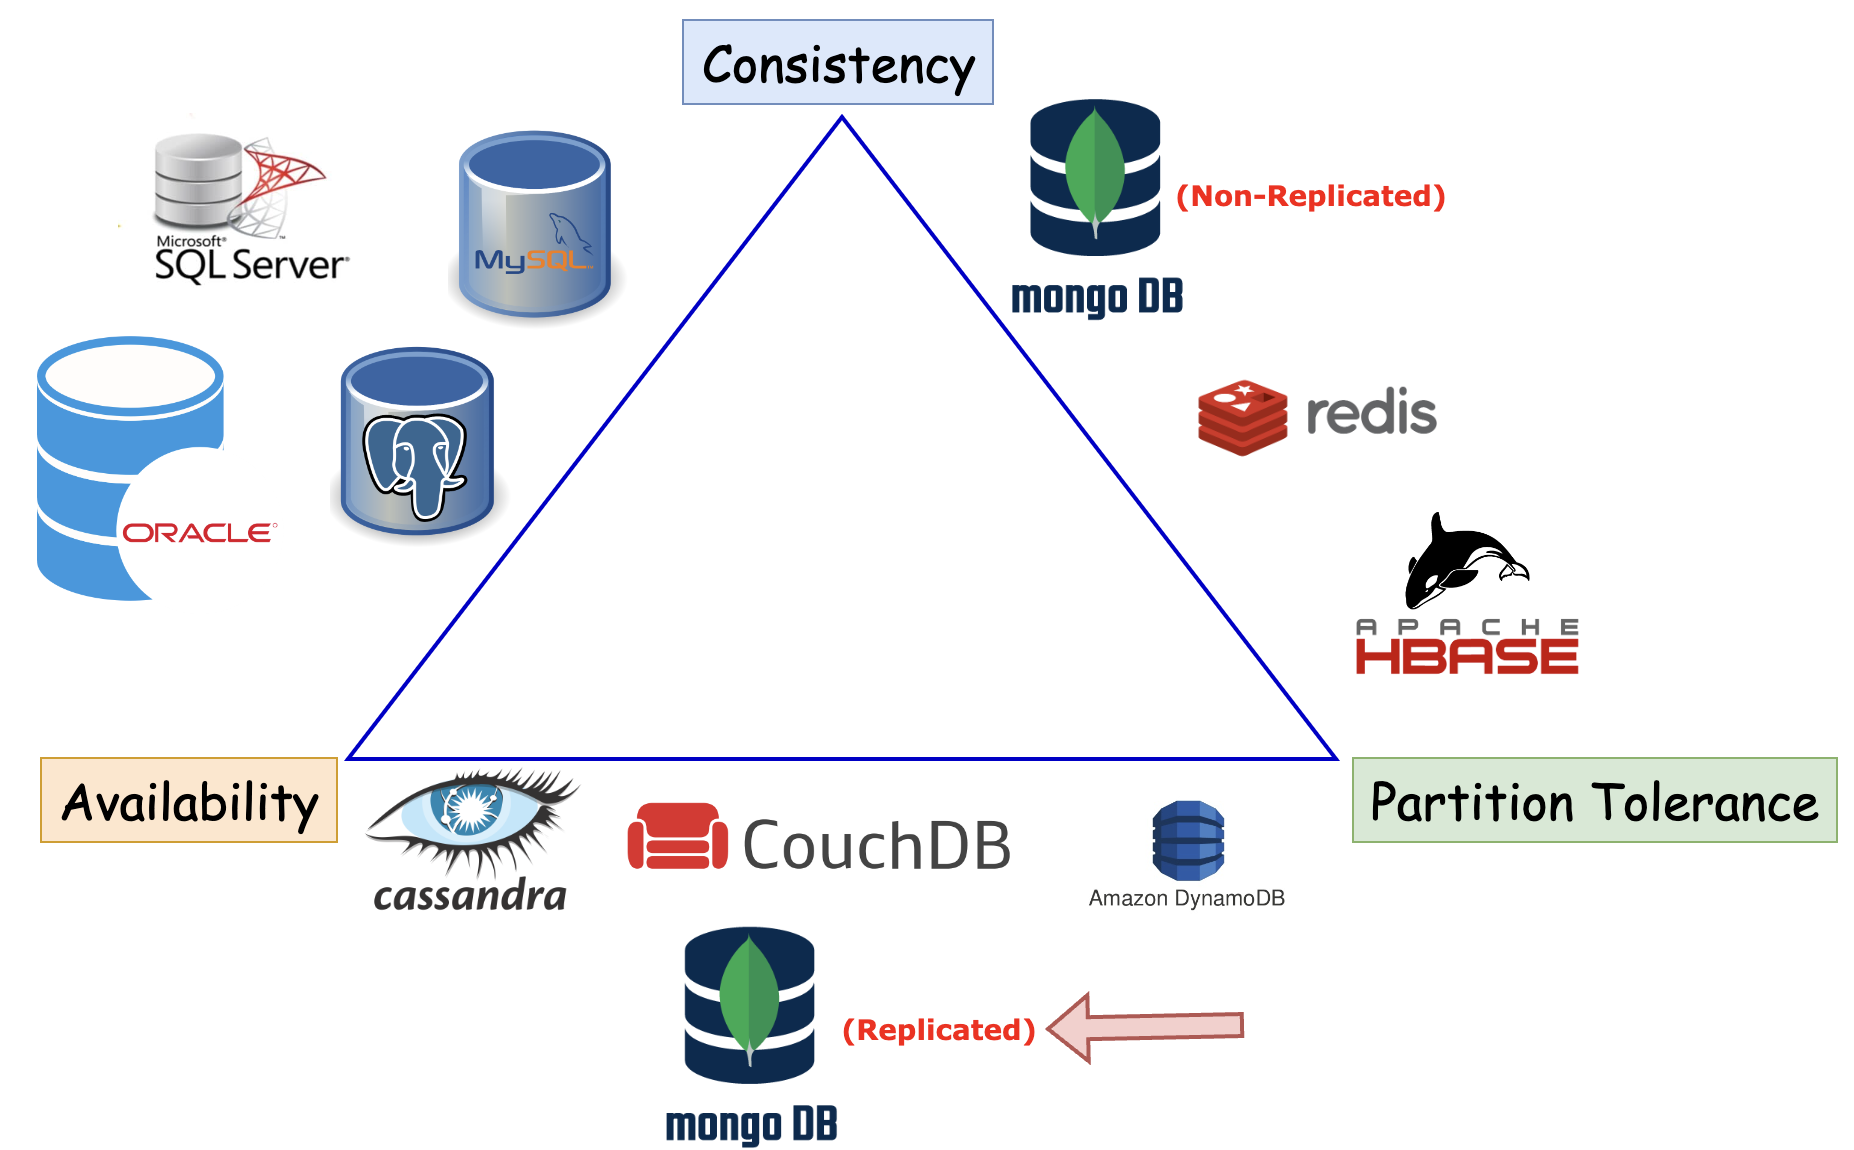
\includegraphics[width=0.8\textwidth]{img/db-cap-theorem.png}
  \end{center}
\end{frame}


\section{High Availability and Scalability}
\begin{frame}{High Availability and Scalability}
  \begin{itemize}
    \item Load Balancer
    \item API Gateway
    \item Rate Limiter
    \item[] 
    		\begin{center}
   	 		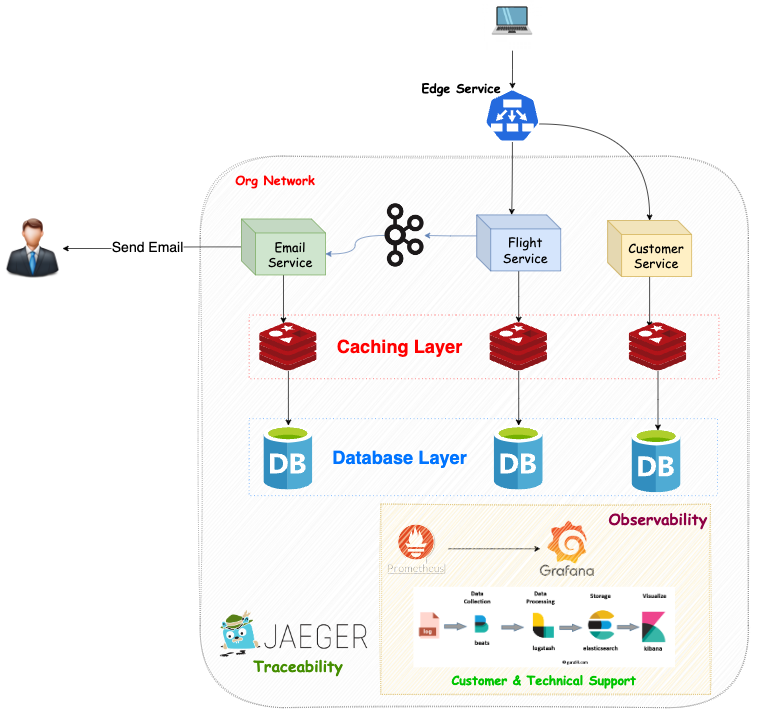
\includegraphics[width=0.7\textwidth, height=60mm, scale=2]{img/hld-latest.png}
  		\end{center}
  	\end{itemize}
\end{frame}

\section{Scalability}
\begin{frame}{Horizontal Scaling vs Vertical Scaling}
	\begin{center}  
  		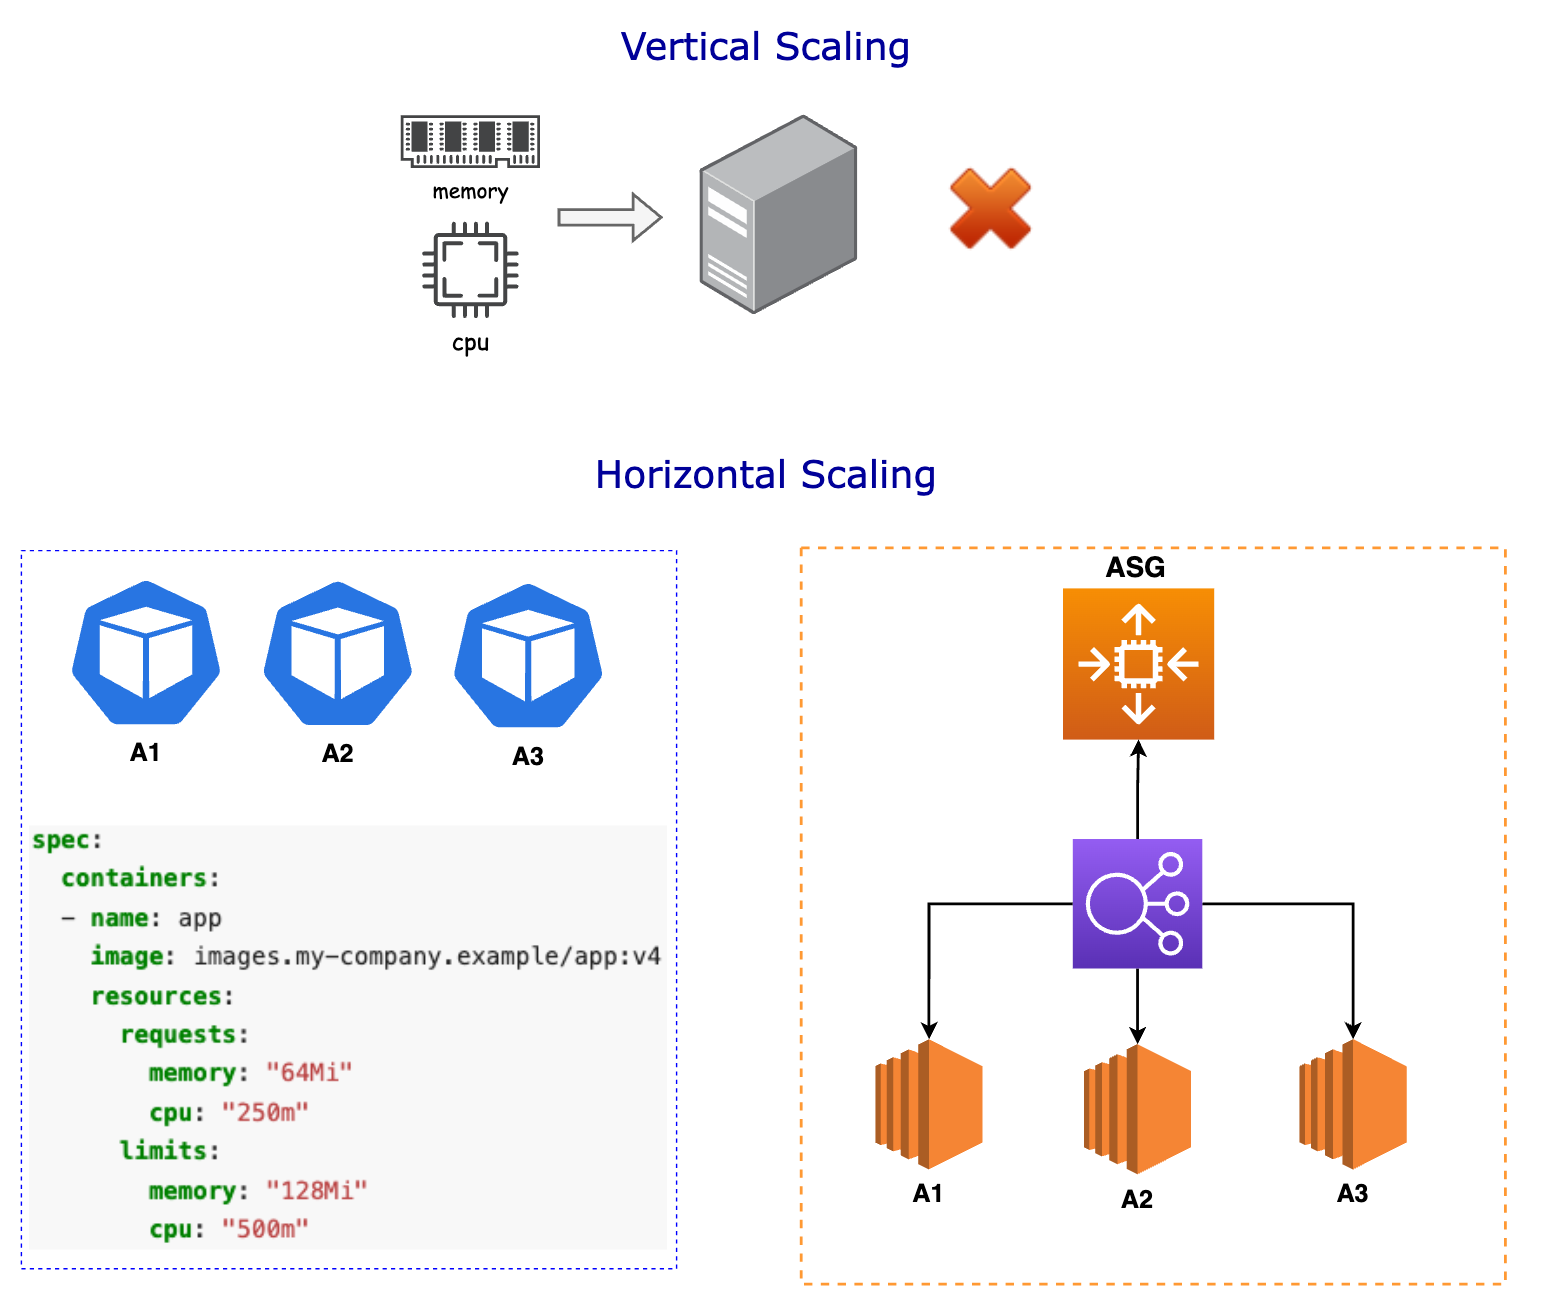
\includegraphics[scale = 0.3]{img/scaling.png}
  	\end{center}
\end{frame}

\section{Resiliency}
\begin{frame}{Resiliency}
    		\begin{center}
   	 		\lstinputlisting[language=python]{application.yml}
  		\end{center}
\end{frame}

\section{Data Replication}
\begin{frame}{Data Replication}
        \begin{center}
   	 		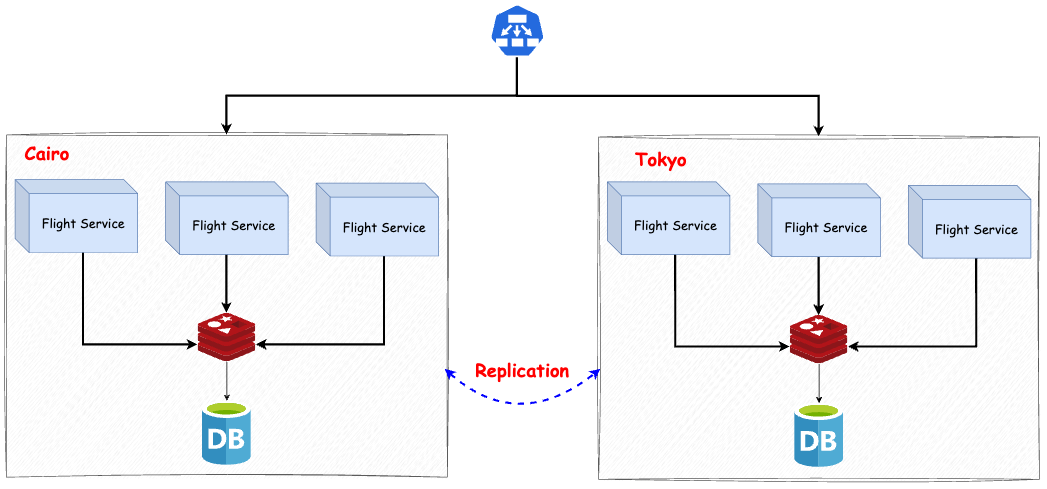
\includegraphics[width=0.8\textwidth, height=60mm, scale=1]{img/DR.png}
  		\end{center}
\end{frame}

\section{Distributed Messaging Systems}
\begin{frame}{Distributed Messaging Systems}
  \begin{itemize}
    \item Introduction to distributed messaging systems
    \item Overview of Kafka and RabbitMQ
  \end{itemize}
\end{frame}

\begin{frame}{RabbitMQ vs Kafka}
        \begin{center}
   	 		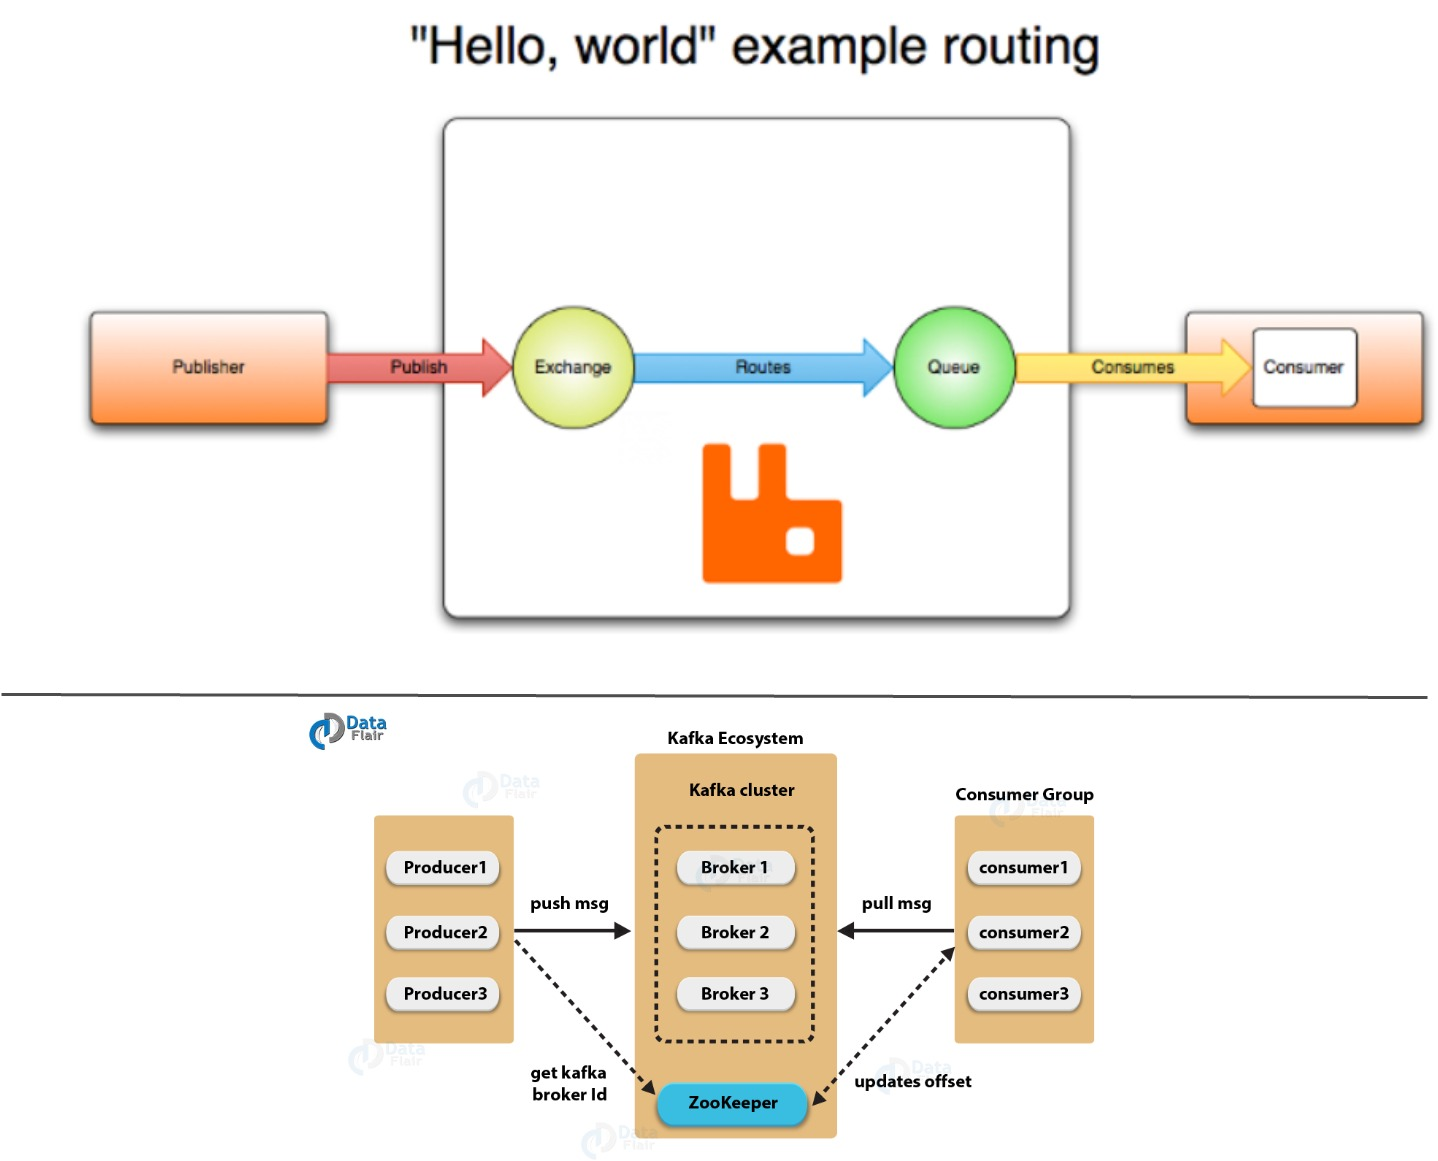
\includegraphics[width=120mm, height=70mm, scale=1]{img/kafkavsrmq.jpg}
  		\end{center}
\end{frame}

\begin{frame}{Data Replication: CDC}
\small In databases, \textbf{change data capture (CDC)} is a set of \textit{software design patterns} used to determine and track the data that has changed (the "deltas") so that action can be taken using the changed data.
        \begin{center}
   	 		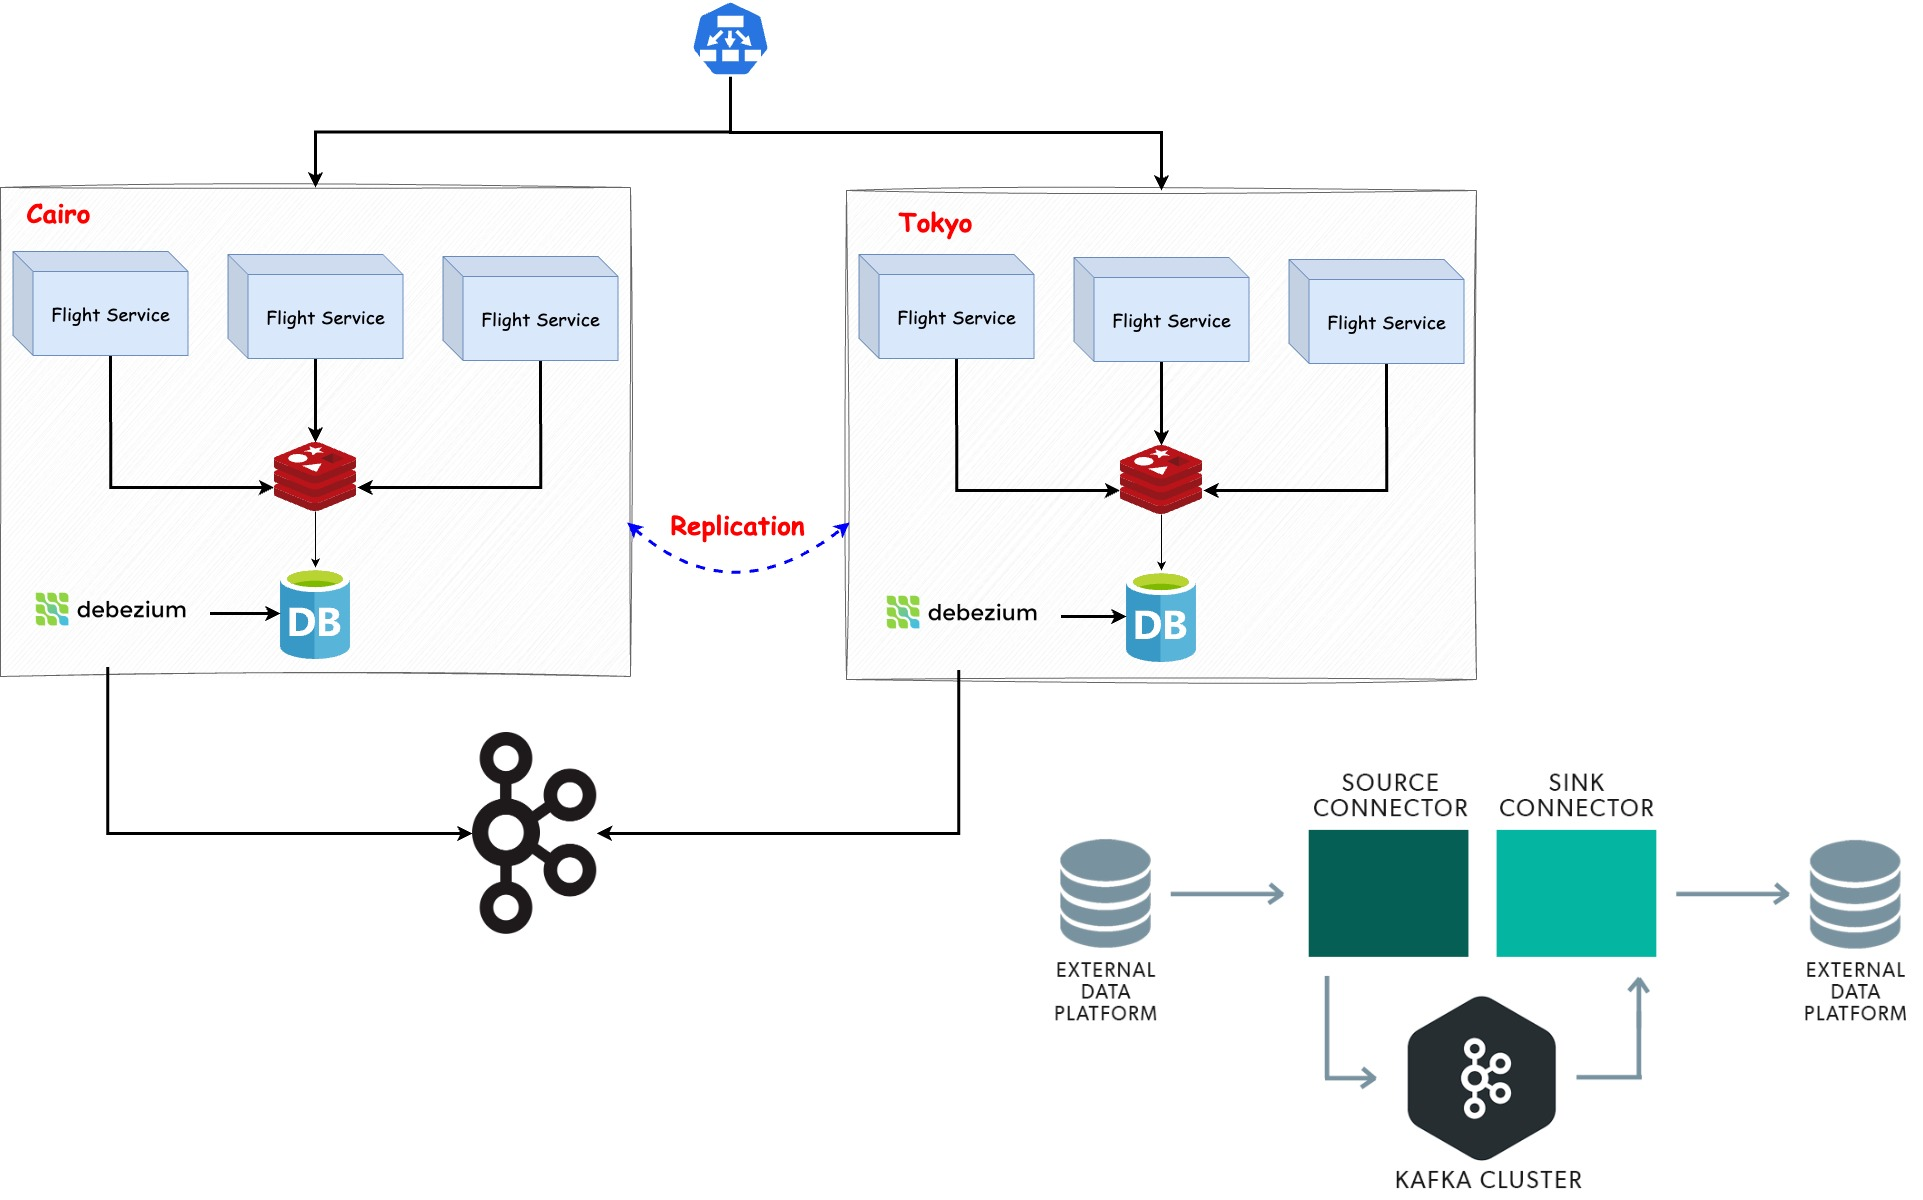
\includegraphics[width=0.8\textwidth, height=60mm, scale=1]{img/kafka-connect1.jpg}
  		\end{center}
\end{frame}

\begin{frame}{Data Replication: CDC}
	\begin{center}
   	 		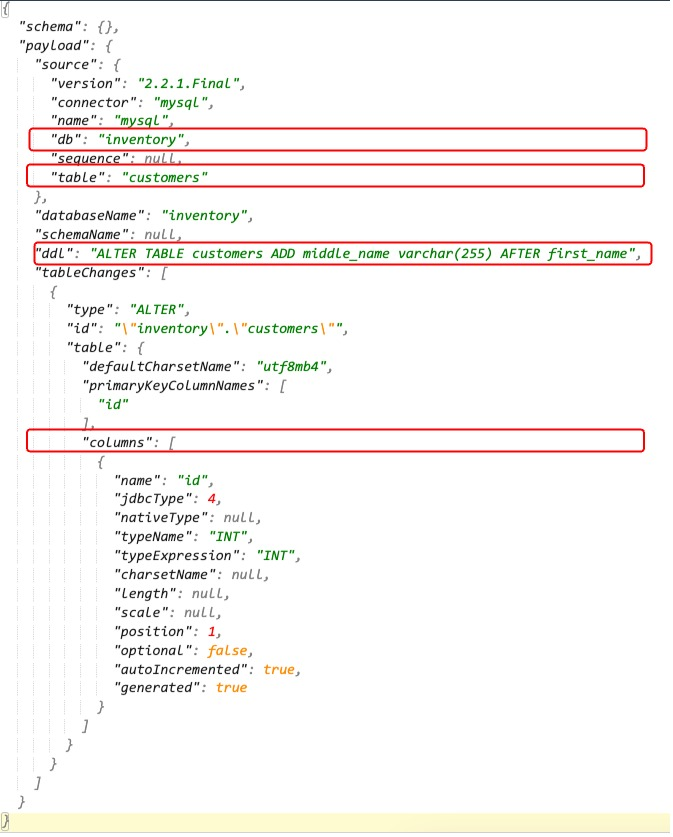
\includegraphics[width=0.7\textwidth, height=80mm, scale=2]{img/cdc-example.jpg}
  		\end{center}
\end{frame}


\begin{frame}{Distributed Messaging Systems}
  \begin{itemize}
    \item Introduction to distributed messaging systems
    \item Overview of Kafka and RabbitMQ
    \item Comparison between Kafka and RabbitMQ:
  \end{itemize}

  \begin{table}[h]
    \centering
    \footnotesize
    \renewcommand{\arraystretch}{1.5}
    \begin{tabular}{|p{0.45\textwidth}|p{0.45\textwidth}|}
      \hline
      \rowcolor[RGB]{232,232,232}
      \textbf{\textcolor{blue}{Kafka}} & \textbf{\textcolor{red}{RabbitMQ}} \\
      \hline
      High-throughput, fault-tolerant distributed streaming platform. &
      Robust and flexible messaging broker. \\
      \hline
      Emphasizes real-time event streaming and data pipeline use cases. &
      Implements Advanced Message Queuing Protocol (AMQP). \\
      \hline
      Provides strong durability and replication guarantees. &
      Focuses on message queuing and asynchronous communication. \\
      \hline
      Scales horizontally to handle large-scale data streams. &
      Provides various messaging patterns (e.g., publish-subscribe, point-to-point). \\
      \hline
      Supports complex event processing with built-in stream processing. &
      Offers pluggable message durability, routing, and acknowledgement mechanisms. \\
      \hline
    \end{tabular}
  \end{table}
\end{frame}


\section{Distributed Key-Value Stores}
\begin{frame}{Distributed Key-Value Stores}
	  
  \begin{itemize}
  	\item[] A type of NoSQL DBs, the idea behind having \textbf{it} is having an extremely fast mechanism for retrieving the data.
    \item Introduction to distributed key-value stores (e.g., Redis, Memcached)
    \item Data partitioning and replication techniques
    \item Consistency and availability trade-offs
  \end{itemize}
\end{frame}


\begin{frame}{Distributed Key-Value Stores: Memcached vs Redis}
	
\includegraphics[width=0.1\textwidth]{img/memcached_image.png}		\hfill
    
\includegraphics[width=0.1\textwidth]{img/redis_image.png}
  \begin{table}[h]
    \centering
    \footnotesize
    \renewcommand{\arraystretch}{1.5}
    \begin{tabular}{|p{0.45\textwidth}|p{0.45\textwidth}|}
      \hline
      \rowcolor[RGB]{232,232,232}
      \textbf{\textcolor{blue}{Memcached}} & \textbf{\textcolor{red}{Redis}} \\
      \hline
      In-memory key-value store primarily designed for caching.
      & 
      In-memory key-value store with additional data structures and functionality.
      \\
      \hline
      Supports simple key-value operations like GET, SET, DELETE. &
      Offers a rich set of data structures (strings, lists, sets, hashes, sorted sets). \\
      \hline
      Lacks built-in persistence mechanisms. &
      Provides persistence options (snapshotting, append-only file, replication). \\
      \hline
      Does not support complex queries or secondary indexes. &
      Supports more advanced operations like sorting, ranking, and filtering. \\
      \hline
      Focuses on high performance and low latency. &
      Balances performance with additional functionality and data structures. \\
      \hline
      No built-in way of replication, requires additional component. &
      Come with out-of-the-box replication using cluster, and as feature with \textbf{Sentinel}. \\
      \hline
    \end{tabular}
  \end{table}
\end{frame}

\section{Consensus}
\begin{frame}{Consensus}
		\begin{center}
   	 		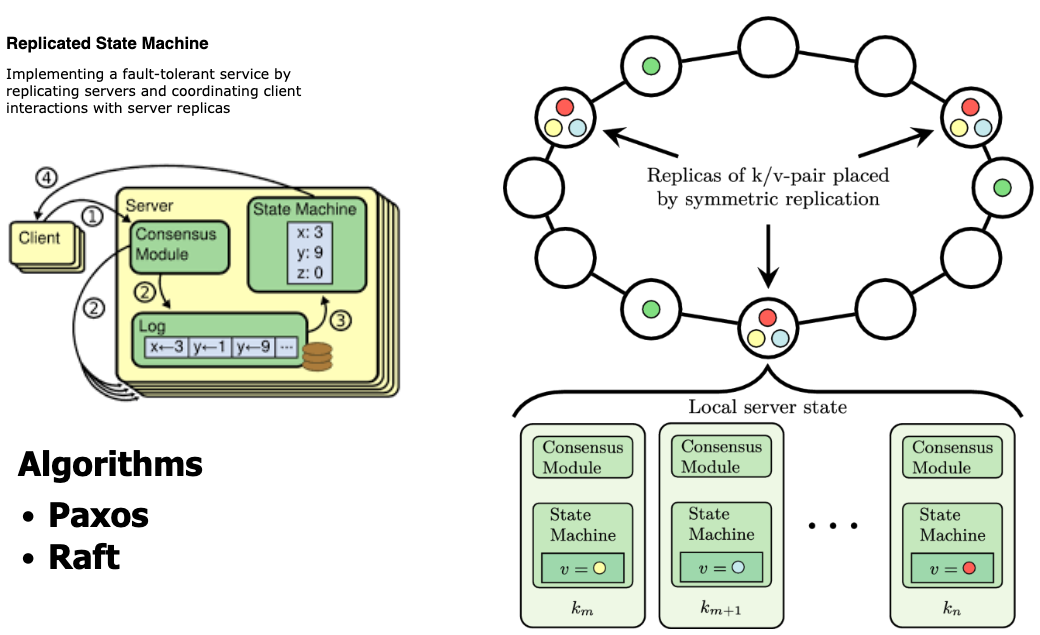
\includegraphics[width=0.9\textwidth, height=70mm, scale=1]{img/consensus.PNG}
  		\end{center}
\end{frame}

\section{Distributed System Security}
\begin{frame}{Distributed System Security}
  \begin{center}
   	 		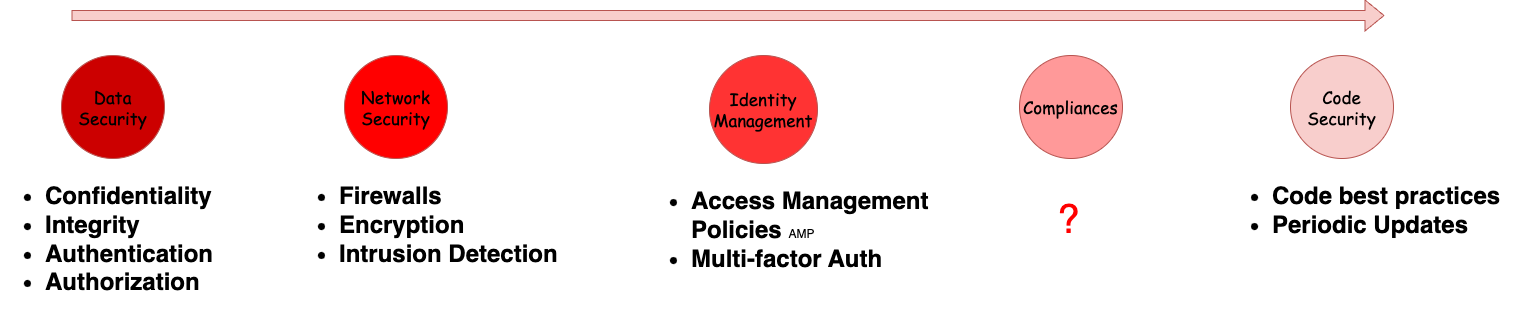
\includegraphics[width=0.9\textwidth, height=30mm, scale=1]{img/security.PNG}
  \end{center}
\end{frame}
\begin{frame}{Distributed System Security}
		\begin{center}
   	 		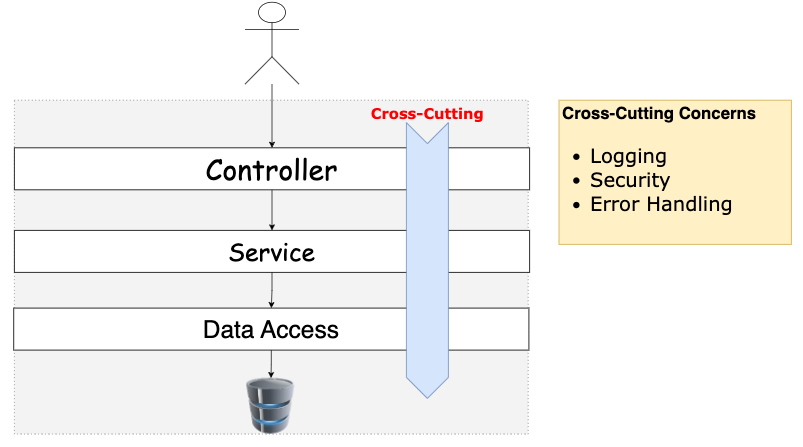
\includegraphics[width=0.7\textwidth, height=60mm, scale=1]{img/cross-cutting.png}
  		\end{center}
\end{frame}

\section{Distributed System Monitoring}
\begin{frame}{Distributed System Monitoring}
  \begin{itemize}
    \item Log aggregation and distributed tracing
    \item Metrics collection and monitoring tools (e.g., Prometheus, Grafana)
    \item Anomaly detection and performance optimization
  \end{itemize}
\end{frame}

\begin{frame}{API Documentations}
  \begin{center}
    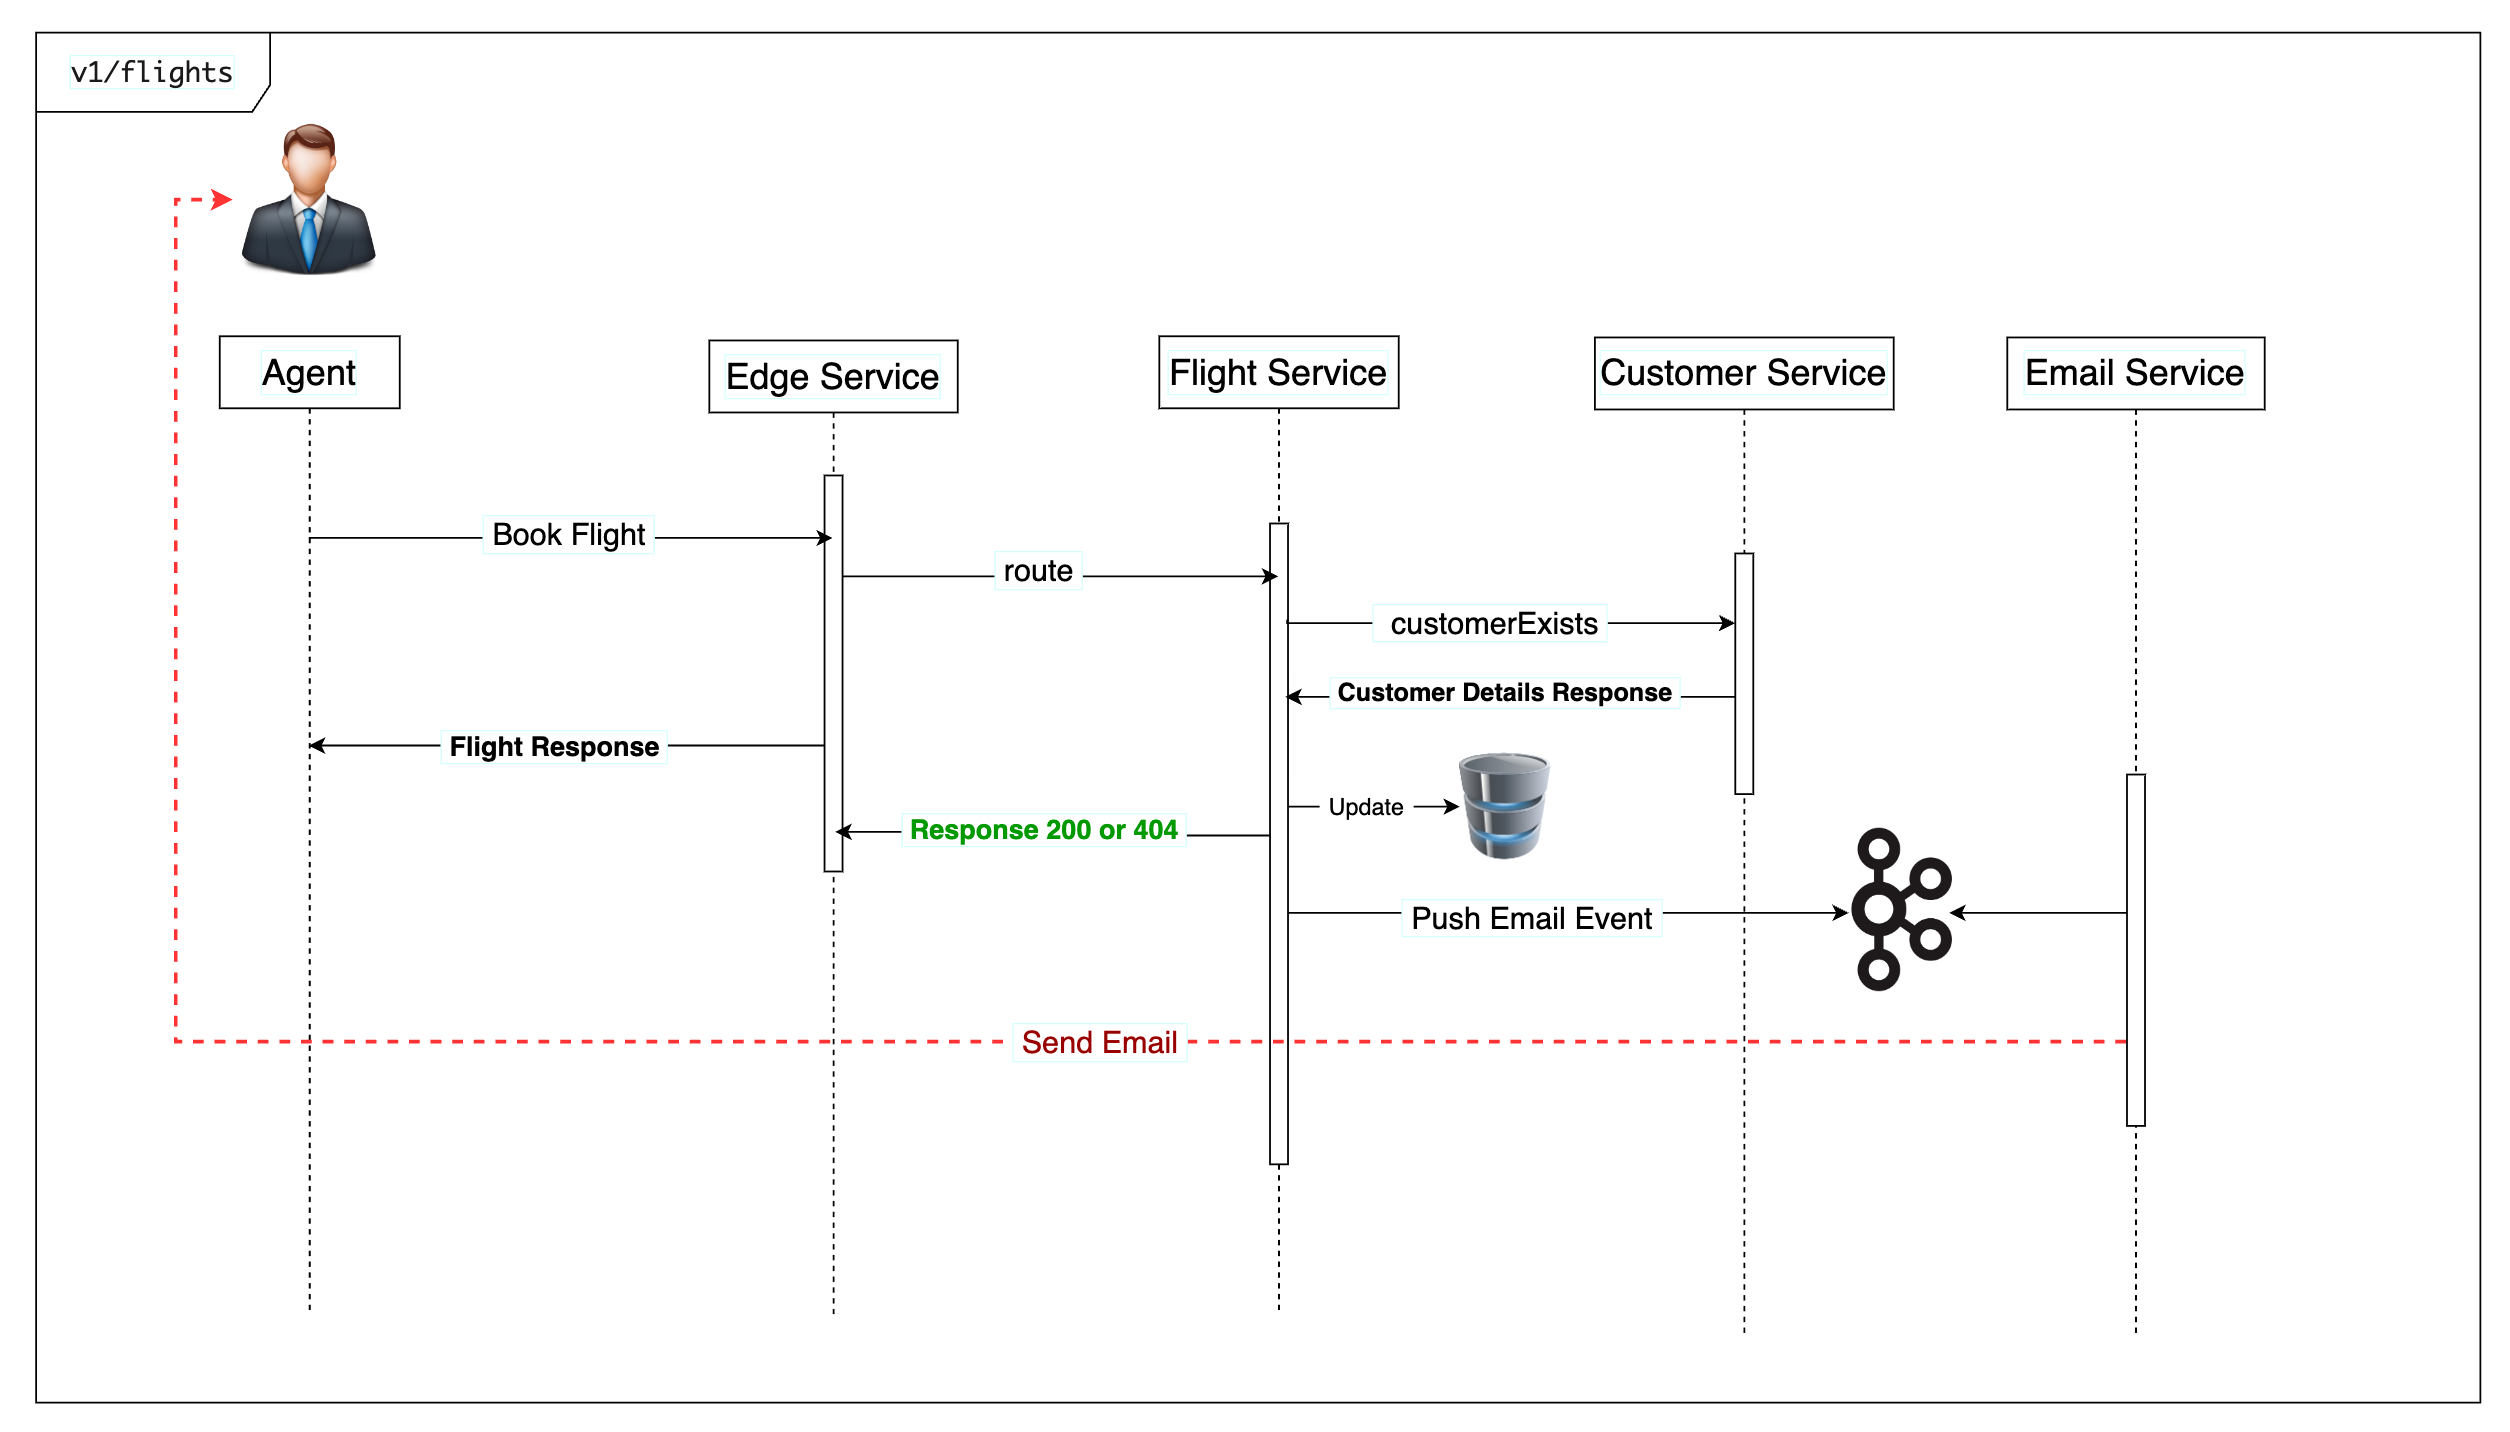
\includegraphics[width=0.9\textwidth]{img/sd.png} 
  \end{center} 
\end{frame}

\section{Conclusion}
\begin{frame}{Conclusion}
  \begin{itemize}
    \item Recap of distributed systems concepts
    \item Overview of various distributed systems topics
    \item Further resources for exploring distributed systems in depth
  \end{itemize}
\end{frame}

\end{document}
